\documentclass{thesisbyxetex}

\usepackage[xetex]{graphicx}	%	Подключаем графику
\usepackage{mathtools}		% 	Подключаем математические символы

\usepackage{amsmath}

\usepackage{fontspec}
\usepackage{unicode-math}
\usepackage{xunicode}
\usepackage{xltxtra}% говорят что не нужен

%для борьбы с переполнениями за счет разреженных слов в абзаце
\emergencystretch=25pt

\usepackage{polyglossia}
\setdefaultlanguage[spelling = modern]{russian}
\setotherlanguage{english} 
\defaultfontfeatures{Scale = MatchLowercase,Ligatures=TeX}  %% устанавливает поведение шрифтов по умолчанию  

\setmainfont{XITS}
\setmathfont{XITS Math}
\newfontfamily\cyrillicfont{XITS}
\setsansfont[Mapping=tex-text]{Nimbus Sans L}
\setmonofont{Nimbus Mono L}


\usepackage{enumitem}	
\setlist{nolistsep}	% отступы между элементами перечесления

\usepackage[unicode, pdfborder={0 0 0 0}]{hyperref}

\usepackage[autostyle]{csquotes}
\usepackage[%parentracker=true,
  backend=biber,
  hyperref=auto,
  language=auto,
  autolang=other,
  style=gost-numeric,
]{biblatex}
\addbibresource{bibliography.bib}

\begin{document}

\hypersetup{
pdftitle = {Курсовая работа},
pdfauthor = {Кочурко Александр Александрович},
pdfsubject = {курсовая},
pdfkeywords = {графический движок, язык D, курсовая}
}% End of hypersetup

\begin{titlepage}
\newpage

\begin{center}
БЕЛОРУССКИЙ ГОСУДАРСТВЕННЫЙ УНИВЕРСИТЕТ \\
МЕХАНИКО-МАТЕМАТИЧЕСКИЙ ФАКУЛЬТЕТ\\
КАФЕДРА ВЕБ-ТЕХНОЛОГИЙ И КОМПЬЮТЕРНОГО МОДЕЛИРОВАНИЯ
\end{center}
 
\vspace{14em}

\begin{center}
Курсовая работа
\end{center}

\begin{center}
\Large \textbf{Название}
\end{center}

\vspace{11em}
 
\begin{flushright}
\parbox{0.45\textwidth}{
Научный руководитель:
\vspace{0.25em}

Станкевич Алексей Александрович
\vspace{2em}

Исполнитель:
\vspace{0.25em}

студент 2 курса, 2 группы

Кочурко Александр Александрович
}%end parbox
\end{flushright}
 
\vspace{\fill}

\begin{center}
Минск 2014
\end{center}

\end{titlepage} 
	% Титульный лист
\tableofcontents 	% Оглавление, которое генерируется автоматически
\chapter*{��������}
����������� ������ (����. graphics engine) � ����������� �����������,
�������� ������� �������� �������� ������������ (���������) ���������� ��� ���������
������������ �������. ����������� ������, �������������� � ���������� �� ������ � ������������ ��������,
������ ���������� ������������, �������������� ��� ����������������.
���� �������� ������������ ������ ������������, ��� �������, � ������������ �����.

�������� ������� ������� ����������� ������� �� ��������� ������� � ���, ��� ������ ������ �������� � ������ ��������� �������,
����� ��� ������ ����� ������� ����� �������
�� ����� ������ �����������. ����� ������������ �������� �������� ��, ��� ����������� ������ ���������� ������������ � �������
����������� ����������� (GPU), ��������� ���������� ������ ����������� ���������� (CPU).

�������� ���� ������ ������ ����������� � ���������� ����������, ���������� �����������, ����������� ���
�������� �������� ������������ ������. ���������� ������ ������ �������� � ������������� �������� ������������� ������������.

��������� ����������� � ����������� ����������:
\begin{enumerate}
\item ��������� ��������.
\item ��������� �����.
\item ��������� �������.
\item �������� � ����� ����������� ������.
\item ��������������������.
\end{enumerate}
����� ����� ������ �������� ������������ ������� ��������� ������ ������������ OpenGL.

������ ����������� �� ����� D - ��������-���������������, ������������������� ����� ����������������, ���������� �������� �������� ������ �����.  
\chapter{Трёхмерная графика}
\section{Основные понятия и существующие технологии}
Трёхмерная графика - совокупность приемов и инструментов, предназначенных для отображения объёмных объектов.


Трёхмерное изображение на плоскости отличается от двумерного тем, что включает построение 
геометрической проекции трёхмерной модели сцены на плоскость. Поскольку мы говорим 
о компьютерной графике, под плоскостью подразумевается экран монитора.
Для изображения трехмерных объектов на экране монитора требуется проведение серии процессов 
(обычно называемых конвейером) с последующей трансляцией результата в двумерный вид. 
Первоначально, объект представляется в виде набора точек, или координат, в трехмерном пространстве. 
Трехмерная система координат определяется тремя осями: горизонтальной, вертикальной и осью глубины, 
обычно называемых, соответственно, осями x, y и z. Соединив определённым образом вершины объекта, 
мы получим его каркасную модель. Каркасная модель определяет области, 
которые могут быть заполнены цветом, текстурами и освещаться лучами света.


Очевидно, что для рендеринга трехмерного объекта требуется много вычислений. Если объект движется, 
объём вычислений увеличивается. Поэтому большую часть вычислений, связанных 
с обработкой объекта трёхмерной сцены, берёт на себя графический процессор (Graphics Processing Unit).



\subsection{OpenGL}
OpenGL (Open Graphics Library) ---  спецификация, определяющая независимый от языка программирования 
платформонезависимый программный интерфейс, включающий более 300 функций для рисования сложных 
трёхмерных сцен из простых примитивов. На основе этой спецификации производители графических процессоров
создают реализации --- библиотеки функций, соответствующие набору функций спецификации.

OpenGL не включает функций для создания окон или для захвата пользовательского ввода. Поэтому существует 
ряд библиотек, обеспечивающих такие возможности, как создание интерфейса пользователя, настройка контекста 
рисования и обработка сообщений от устройств ввода-вывода.  Примерами таких библиотек могут служить GLUT, SDL, GLFW и т.д.


\section{Процесс визуализации объектов}
\subsection{Представление объекта в памяти компьютера}
Рассмотрим подробнее процесс рендеринга объектов. В настоящее время в компьютерной графике популярно представление
поверхностей в виде полигональной сетки (совокупности вершин, рёбер и граней, которые определяют форму многогранного объекта). 
Гранями в компьютерных играх, как правило, являются треугольники, поскольку графические процессоры 
способны на аппаратном уровне быстро обрабатывать этот примитив. У каждой вершины треугольника есть так называемые 
атрибуты, среди которых, естественно, координаты вершины в пространстве, вектор нормали, координаты текстуры и т.д. 
Таким образом описание объекта сводится к описанию атрибутов вершин треугольников, из которых состоит его поверхность. 
Атрибуты вершин принято хранить в массиве (в одном или нескольких для каждого из атрибутов). Далее, 
используя функции OpenGL, следует сообщить графическому процессору о созданном объекте и вызвать функцию отрисовки, 
которая в соответствии с определёнными правилами отрисует вершины в таком порядке, 
в каком они расположены в описанном массиве. Часто возникает ситуация, когда вершина принадлежит нескольким треугольникам, 
а значит при вышеописанном подходе её необходимо дублировать столько раз, сколько треугольников её содержит. 
В объектах с большим количеством треугольников это может привести к бессмысленной трате памяти, поэтому 
часто используется так называемый буфер индексов - массив, каждый элемент которого есть индекс определённой вершины
в массиве вершин. Можно вызвать функцию отрисовки таким образом, чтобы графический процессор отрисовывал вершины в 
том порядке, в котором расположены их индексы в буфере индексов.
\subsection{Процесс обработки вершин. Шейдеры}
При вызове функции отрисовки каждая точка, принадлежащая текущему объекту, проходит несколько этапов обработки, 
и только после этого проецируется на экран. Эти этапы, как было отмечено ранее, в совокупности составляют 
графический конвейер, который представлен следующим образом:
\begin{enumerate}
\item Вершинный процессор
\item Геометрический процессор
\item Клиппер (обрезает те фрагменты, которые не попадают на экран
\item Фрагментный процессор
\end{enumerate}


Далее следует ввести понятие шейдера

\textbf{Шейдер} --- программа для одной из ступеней графического конвейера, используемая в трёхмерной графике 
для определения окончательных параметров объекта или изображения.
Существует три вида шейдеров: вершинный (оперирует данными, сопоставленными с вершинами треугольников), 
фрагментный (работает с фрагментами растрового изображения) и геометрический (способен за одно выполнение 
обработать целый треугольник). Есть несколько языков программирования, разработанных для создания шейдеров. 
Наиболее популярным является GLSL (The OpenGL Shading Language). Код, написанный на GLSL, обрабатывается компилятором, 
который является частью драйвера видеокарты, затем используется видеопроцессором. Спецификация OpenGL предоставляет 
функции для загрузки и компиляции шейдеров, а также для обмена данными между шейдером и основным приложением.

Итак, каждый шейдер выполняется на соответствующем этапе графического конвейера, затем осуществляется рендеринг изображения.

\section{Преобразования координат вершин}
Данный раздел представляет наибольший интерес, поскольку преобразования координат тесно связаны с линейной алгеброй. 
Следует отметить, что несмотря на возможность представления поворота и масштабирования матрицами размера \begin{math}3\times3\end{math}, 
перемещение представить матрицей такого размера невозможно, поэтому принято использовать матрицы размера \begin{math}4\times4\end{math}. 
Далее все преобразования рассматриваются в случае трёхмерного пространства.
\subsection{Масштабирование}
Масштабирование - наиболее простое преобразование, которое может быть представлено матрицей вида
\begin{equation}
\mathrm{S} = 
  \begin{pmatrix}
    \lambda & 0 & 0 & 0 \\
    0 & \lambda & 0 & 0 \\
    0 & 0 & \lambda & 0 \\
    0 & 0 & 0 & 1
  \end{pmatrix},
\end{equation}
\begin{eqrem}
\begin{math} \lambda \end{math} --- коэффициент масштабирования.
\end{eqrem}

\subsection{Вращение}
Вращение есть произведение матриц поворота вокруг некоторых ортогональных осей на 
определённый угол (в данном случае - вокруг координатных осей):

\begin{equation}
\mathrm{R}_x = 
  \begin{pmatrix}
    1 & 0  & 0 & 0\\
    0 & \cos\varphi & -\sin\varphi & 0\\
    0 & \sin\varphi & \cos\varphi & 0\\
    0 & 0 & 0 & 1
  \end{pmatrix},
\end{equation}

\begin{equation}
\mathrm{R}_y = 
  \begin{pmatrix}
    \cos\psi  & 0 & -\sin\psi & 0\\
    0 & 1 & 0 & 0 \\
    \sin\psi & 0 & \cos\psi & 0\\
    0 & 0 & 0 & 1
  \end{pmatrix},
\end{equation}

\begin{equation}
\mathrm{R}_z = 
  \begin{pmatrix}
    \cos\eta & -\sin\eta & 0 & 0 \\
    \sin\eta & \cos\eta  & 0 & 0\\
    0 & 0 & 1 & 0\\
    0 & 0 & 0 & 1
  \end{pmatrix},
\end{equation}
\begin{eqrem}
\begin{math} \varphi, \psi, \eta\end{math} --- соответственно углы поворота вокруг осей \begin{math}x, y, z\end{math}.
\end{eqrem}

Результирующее преобразование: \begin{math}\mathrm{R} = \mathrm{R}_z \mathrm{R}_y \mathrm{R}_x\end{math}.

\subsection{Перемещение}
Матрица перемещения достаточно простого вида:

\begin{equation}
\mathrm{T} = 
  \begin{pmatrix}
    1 & 0  & 0 & x\\
    0 & 1 & 0 & y\\
    0 & 0 & 1 & z\\
      0 & 0 & 0 & 1
  \end{pmatrix},
\end{equation}
\begin{eqrem}
\begin{math} x, y, z \end{math} - координаты вектора перемещения.
\end{eqrem}

\subsection{Проекция перспективы}
При проецировании трёхмерного пространства на двумерную плоскость для реалистичности изображения следует сохранять его глубину.
Это достаточно нетривиальная задача. Для её решения используется преобразование, известное как проекция перспективы. 
Кроме упомянутой задачи, проекция перспективы решает и другую: в современных мониторах ширина экрана, как правило, больше, чем высота. 
В то же время графический процессор обрабатывает вершины с координатами, лежащими в отрезке [-1.0, 1.0] по всем координатным осям. 
Это означает, что, например, квадрат будет отображен как прямоугольник. Рассматриваемое преобразование призвано решать эту проблему.
Для построения проекции перспективы используются следующие входные данные:

\begin{enumerate}
\item \begin{math}q\end{math} - соотношение сторон прямоугольной области, на которую будет осуществляться проекция.
\item \begin{math}\alpha\end{math} - угол обзора камеры по вертикали.
\item \begin{math}d_n\end{math} - позиция ближайшей видимой плоскости, перпендикулярной оси \begin{math}z\end{math}.
\item \begin{math}d_f\end{math} - позиция самой дальней видимой плоскости, перпендикулярной оси \begin{math}z\end{math}.
\end{enumerate}

Рассмотрим этапы построения матрицы данного преобразования.
(далее --- проецированных координат). Для начала следует найти расстояние от камеры до плоскости проекции, используя угол обзора по вертикали:

\begin{equation}d = \frac{1}{\tan{\frac{\alpha}{2}}} \end{equation}

Затем можно приступить непосредственно к подсчёту проецированных координат \begin{math}x, y\end{math}.
Пусть обрабатывается вершина с координатами \begin{math}(x, y, z)\end{math}. Нужно найти \begin{math}(x_p, y_p)\end{math} - соответствующие 
координаты на плоскости проекции.
Рассмотрим следующий рисунок:
  \begin{figure}\begin{center}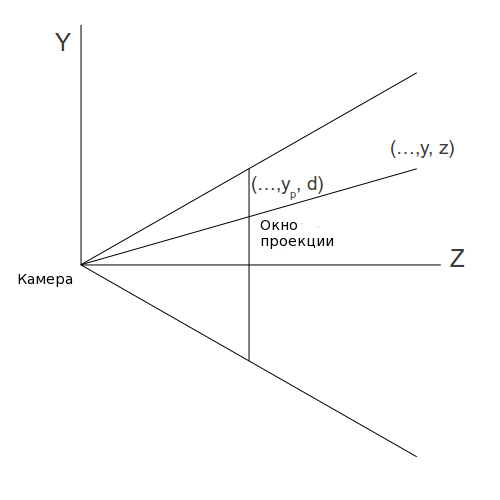
\includegraphics[scale = 0.5]{cam.png} \end{center}\end{figure}
Согласно правилу подобных треугольников:
  \begin{equation}y_p = \frac{yd}{z} = \frac{y}{z\tan{\frac{\alpha}{2}}},    x_p = \frac{xd}{z} = \frac{x}{z\tan{\frac{\alpha}{2}}}\end{equation}
Ширина и высота окна проекции равны, очевидно, \begin{math}2q\end{math} и \begin{math}2\end{math} соответственно. Точка в пространстве попадает в окно проекции, 
если она проецируется в точку с координатами \begin{math}x_p\in[-q, +q]\end{math},
   \begin{math}y_p\in[-1, 1]\end{math}. Координата \begin{math}y_p\end{math} нормирована, осталось пронормировать координату \begin{math}x_p\end{math}, поделив 
   на соотношение сторон \begin{math}q\end{math}. Теперь точка, с координатой \begin{math}x = q\end{math} имеет координату \begin{math}x_p = 1.0\end{math}, 
   следовательно располагается на правой границе экрана.

В результате получили следующие выражения для \begin{math}x_p\end{math} и \begin{math}y_p\end{math}:
 \begin{equation}y_p = \frac{y}{z\tan{\frac{\alpha}{2}}},    x_p = \frac{x}{qz\tan{\frac{\alpha}{2}}}\end{equation}
   В обоих выражениях присутствует множитель \begin{math}\frac{1}{z}\end{math} Но координата \begin{math}z\end{math} меняется от вершины 
   к вершине, поэтому этот множитель нельзя поместить в матрицу преобразования, применяемую ко всем вершинам. Возникшая проблема в OpenGL 
   решается следующим образом: умножение вектора позиции вершины на \begin{math}\frac{1}{z}\end{math} выполняется графическим процессором после
   прохождения вершинного шейдера, а значит из выражений для \begin{math}x_p\end{math}, \begin{math}y_p\end{math} и последующих этот множитель необходимо убрать.
   Сам процесс умножения на \begin{math}\frac{1}{z}\end{math} называется делением перспективы.

   Далее нужно найти инъективное отображение, переводящее отрезок \begin{math}[d_n, d_f]\end{math} в отрезок \begin{math}[-1, 1]\end{math}. 
   Отображение представляет из себя сжатие \begin{math}[d_n, d_f]\end{math} до отрезка длины \begin{math}2\end{math} с последующим совмещением начала полученного отрезка с \begin{math}-1\end{math}. Теперь ясно, что искомое отображение имеет вид:

   \begin{equation}f(z) = az + b\end{equation}

   , где \begin{math}a, b\end{math} некоторые константы, поиску которых посвящён остаток раздела.
   Известно, что когда \begin{math}f(d_n) = -1, f(d_f) = 1\end{math}. Выполним некоторые вычисления, предварительно разделив 
   \begin{math}f(z)\end{math} на \begin{math}z\end{math}:
   \begin{equation}a + \frac{b}{d_n} = -1 \Rightarrow a = -1 -\frac{b}{d_n} \end{equation}
                                                                             
  
\begin{equation} + \frac{b}{d_f} = 1 \Rightarrow \frac{b}{d_f} - 1 - \frac{b}{d_n} = 1 \Rightarrow b(d_n - d_f) = 2d_n d_f \Rightarrow b = \frac{2d_n d_f}{d_n - d_f}\end{equation}

   \begin{equation}a = -1 - \frac{b}{d_n}  = \frac{-d_n - d_f}{d_n - d_f} \end{equation}

   Имеем:
   \begin{equation}f(z) = \frac{-d_n - d_f}{d_n - d_f}z + \frac{2d_n d_f}{d_n - d_f}\end{equation}


   Теперь можно составить матрицу проекции перспективы (процесс составления матрицы опускается, поскольку не представляет особого интереса).
   В результате получается матрица следующего вида:
\begin{equation}
\mathrm{T} = 
  \begin{pmatrix}
    \frac{1}{q\tan{\frac{\alpha}{2}}} & 0 & 0 & 0 \\
    0 & \frac{1}{\tan{\frac{\alpha}{2}}}  & 0 & 0\\
    0 & 0 & \frac{-d_n - d_f}{d_n - d_f} & \frac{2d_n d_f}{d_n - d_f}\\
    0 & 0 & 1 & 0
  \end{pmatrix},
\end{equation}

\subsection{Камера}
Камера в 3D игре -- это инструмент, позволяющий имитировать разного рода передвижения в пространстве экрана, "око" игрока.
Под имитацией движения в данном случае понимается применение неких преобразований, разговор о которых пойдёт далее.


Положение камеры в пространстве,как и в случае вершин объектов, определяется тремя координатами. Предположим, что камера расположена в начале 
координат, т.е. в точке с координатами \begin{math}(0.0, 0.0, 0.0)\end{math}. Рассмотрим следующий рисунок (вид сверху против направления оси \begin{math}Oy\end{math}:

  \begin{figure}\begin{center}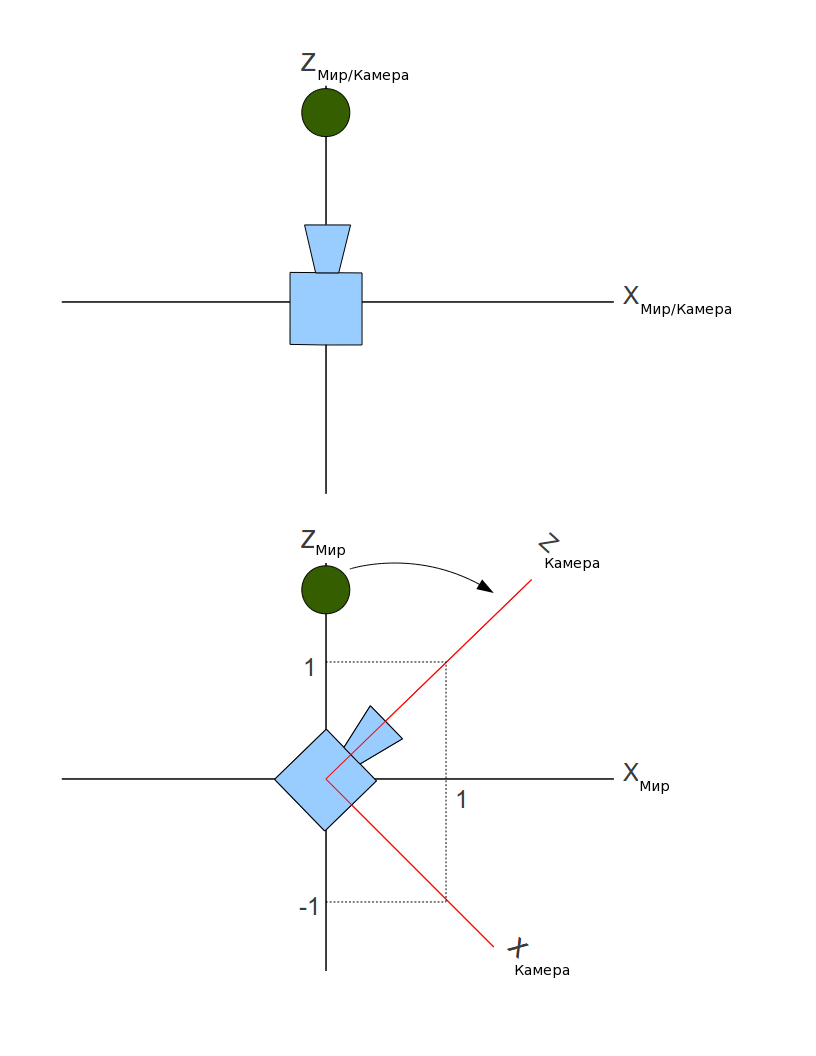
\includegraphics[scale=0.4]{camera.png} \end{center}\end{figure}
  
  
   Сначала камера направлена против оси \begin{math}Oz\end{math}, затем повернута на \begin{math}45^o\end{math} по часовой стрелке. Камера определяет свою собственную систему координат, которая может совпадать с общей, или мировой системой координат (верхнее изображение) либо не совпадать (нижнее). Пространство, заданное направляющими векторами координатных осей мировой системы координат, называют мировым пространством; заданное направляющими векторами  камеры ---  пространством камеры. В пространстве камеры сама камера расположена в начале координат.
    
    Поворот камеры на угол \begin{math}\alpha\end{math} эквивалентен повороту мирового пространства на угол \begin{math}-\alpha\end{math}. Движение мирового пространства всегда противоположно движению камеры.
    Поэтому преобразований, связанных с камерой, два: движение мирового пространства до совпадения координат камеры с началом мировых координат и его поворот в направлении, противоположном вращению камеры.
    
    Движение камеры осуществляется следующим образом: если координаты камеры \begin{math}(x, y, z)\end{math}, то преобразование позиции имеет вид \begin{math}(-x, -y, -z)\end{math}. Объясняется это тем, что камера расположена в мировой системе координат с использованием перемещения, основанного на векторе \begin{math}(x, y, z)\end{math}, поэтому, чтобы поместить ее в начало координат, необходимо преобразование, обратное данному. Таким образом, матрица движения камеры имеет вид:
    
    \begin{equation}
  \mathrm{T_k} = \begin{pmatrix}
    1 & 0  & 0 & x\\
    0 & 1 & 0 & y\\
    0 & 0 & 1 & z\\
      0 & 0 & 0 & 1
  \end{pmatrix}^{-1} = \begin{pmatrix}
    1 & 0  & 0 & -x\\
    0 & 1 & 0 & -y\\
    0 & 0 & 1 & -z\\
      0 & 0 & 0 & 1
  \end{pmatrix}
\end{equation}
     
 Далее осуществляется поворот камеры на некоторые значения, указанные в мировых координатах. О повороте будет упомянуто ниже, для начала следует рассмотреть вопрос о положении объектов в системе координат камеры. Здесь имеет место переход из мировой системы координат в систему координат камеры. Базис мирового пространства может быть представлен ортонормированной системой векторов
 \begin{math}\vec{a_1}(1, 0, 0), \vec{a_2}(0, 1, 0), \vec{a_3}(0, 0, 1), \end{math}, базис пространства камеры тоже можно представить ортонормированной системой \begin{math}\vec{b_1}, \vec{b_2}, \vec{b_3}, \end{math}.
 Матрица перехода от базиса первого базиса ко второму является ортогональной, поскольку оба базиса ортонормированы, и имеет следующий вид:    
 \begin{equation} \mathrm{C}\begin{pmatrix}
    b_{1x} & b_{2x}  & b_{3x} & 0\\
    b_{1y} & b_{2y} & b_{3y} & 0\\
    b_{1z} & b_{2z} & b_{3z} & 0\\
    0 & 0 & 0 & 1
  \end{pmatrix}\end{equation}
  
  По формуле преобразования координат при переходе от базиса \begin{math}\vec{a_i}\end{math} к базису \begin{math} \vec{b_i}\end{math}:
  \begin{math}v_b = C^{-1}v_e\end{math}
  Поскольку для ортогональной матрицы верно \begin{math}C^{-1} = C^{T}\end{math}, имеем:
  
  \begin{equation}
  \begin{pmatrix}
    e_{bx}\\
    e_{by}\\
    e_{bz}\\
    1
  \end{pmatrix} = 
  \begin{pmatrix}
    b_{1x} & b_{1y}  & b_{1z} & 0\\
    b_{2x} & b_{2y} & b_{2z} & 0\\
    b_{3x} & b_{3y} & b_{3z} & 0\\
    0 & 0 & 0 & 1
  \end{pmatrix}
    \begin{pmatrix}
    e_{ax}\\
    e_{ay}\\
    e_{az}\\
    1
  \end{pmatrix}
  \end{equation}
  
  Векторы \begin{math}\vec{b_1}, \vec{b_2},\vec{b_3}\end{math} базиса пространства камеры часто обозначаются соответственно \begin{math}\vec{U}\end{math}, \begin{math}\vec{V}\end{math} и \begin{math}\vec{N}\end{math} соответственно. Вектор \begin{math}\vec{U}\end{math} определяет ось направления, \begin{math}\vec{V}\end{math} - вертикальную ось, \begin{math}\vec{N}\end{math} - горизонтальную.
  Поворот камеры осуществляется в два этапа: поворот вектора U на горизонтальный угол, затем на вертикальный.  
  Для задачи вращения камеры вокруг произвольного вектора есть простое математическое решение - кватернионы. 
   Кватернионы являются 4-х мерным расширением множества комплексных чисел, другими словами ---  это гиперкомплексные числа,  
   то есть кватернион \begin{math}Q\end{math} задаётся четвёркой чисел \begin{math}(x, y, z, w)\end{math}:
   \begin{equation}Q = xi + yj +zk + w\end{equation}
   \begin{eqrem}
    где \begin{math}i^2 = j^2 = k^2 = -1\end{math}
   \end{eqrem}

  Кватернион, сопряжённый данному: \begin{math}Q^{-1} = -xi - yj - zk + w\end{math}
  Нормирование кватернионов определеятся аналогично нормированию векторов.
  
  Формула для подсчета кватерниона \begin{math}w\end{math}, являющегося результатом поворота вектора \begin{math}\vec{v}\end{math} 
  на угол \begin{math}\alpha\end{math} вокруг вектора \begin{math}l\end{math}:
  \begin{equation}w = q\vec{v}q^{-1}\end{equation}\begin{eqrem}где q - кватернион вращения, имеющий вид:
  
  \begin{equation}
  \mathrm{q} = 
    \begin{pmatrix}
    l_x \sin{\frac{\alpha}{2}}\\
    l_y\sin{\frac{\alpha}{2}}\\
    l_z\sin{\frac{\alpha}{2}}\\
    \cos{\frac{\alpha}{2}}
  \end{pmatrix}
  \end{equation}\end{eqrem}  

    После подсчета \begin{math}w\end{math} повернутый вектор имеет координаты \begin{math}(w_x,w_y,w_z)\end{math}.

    Идея поворота камеры состоит в том, чтобы вектор \begin{math}\vec{a}\end{math}, имеющий в пространстве
    камеры координаты \begin{math}(1, 0, 0)\end{math} повернуть на горизонтальный угол вокруг вектора \begin{math}\vec{V}\end{math}, затем перемножить 
    векторно \begin{math}\vec{V}\end{math} и \begin{math}\vec{a}\end{math} для получения нового вектора \begin{math}\vec{U}\end{math} (чтобы новые векторы 
    стали ортогональными), после повернуть \begin{math}\vec{a}\end{math} на вертикальный угол вокруг \begin{math}\vec{U}\end{math} и получить новый вектор
    \begin{math}\vec{V}\end{math} как результат векторного произведения \begin{math}\vec{a} \times \vec{U}\end{math}. Также после каждой из операций новые 
    векторы следует нормировать, поскольку каждый полученный вектор не обязательно единичный.

    \subsection{Результирующее преобразование}
Для получения результирующего преобразования следует переменожить все вышеперечисленные матрицы 
в строго определённом порядке. Нужно иметь ввиду, что вектор позиции вершины умножается на матрицу справа, 
а значит преобразуется каждой матрицей справа налево. В трёхмерной графике принято сначала изменять масштаб объекта, 
затем вращать и после перемещать; после этого могут применяться дополнительные преобразования, связанные с камерой 
и проекцией перспективы. Затем посредством функций из OpenGL нужно отправить получившуюся 
матрицу в вершинный шейдер, где координаты каждой вершины будут на неё умножены.



\printbibliography
\addcontentsline{toc}{chapter}{Литература}

\end{document} 
